\section{Frequency analysis of music}
In this section the recordings of music will undergo frequency analysis, and the goal is to be able to express which frequencies the tones played in the recordings are generally found at. It is expected that both the significant tone and its corresponding harmonics will appear in the frequency spectrum.
   
\subsection{Single tone} \label{sec:single}
Firstly, the tuning of guitar is checked for consistency. The $E_2$ and $E_4$ strings on the guitar (low and high $E$ strings on the guitar, repectively) should vibrate and emit sounds of frequencies of 82.41 Hz and 329.63 Hz, respectively, as seen in table \ref{fig:guitar_frequencies}. Figures \ref{fig:single_low} and \ref{fig:single_high} show the frequency spectra for the recordings of the two tones.
\begin{figure}[H]
\centering
\begin{subfigure}{0.49\textwidth}
\centering
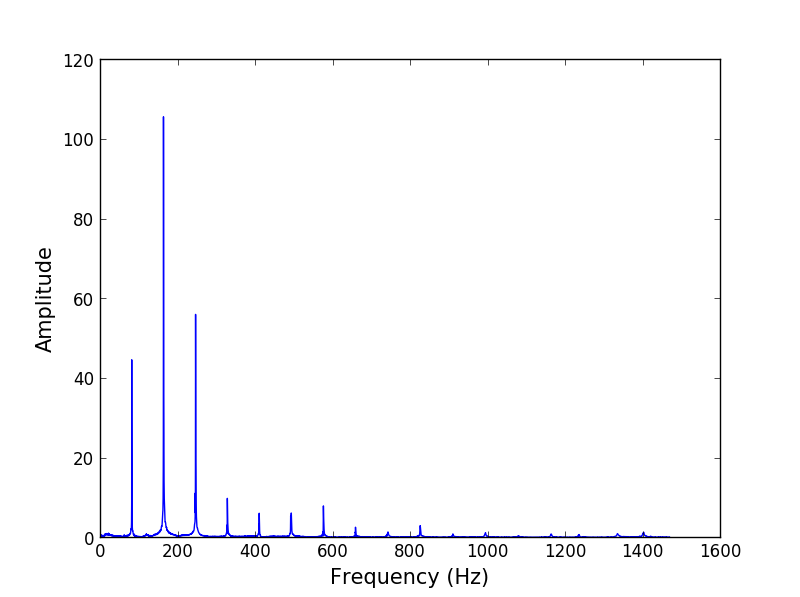
\includegraphics[width=\textwidth]{figures/freqanal/single_low.png}
\caption{$E_2$.}
\label{fig:single_low}
\end{subfigure}
\begin{subfigure}{0.49\textwidth}
\centering
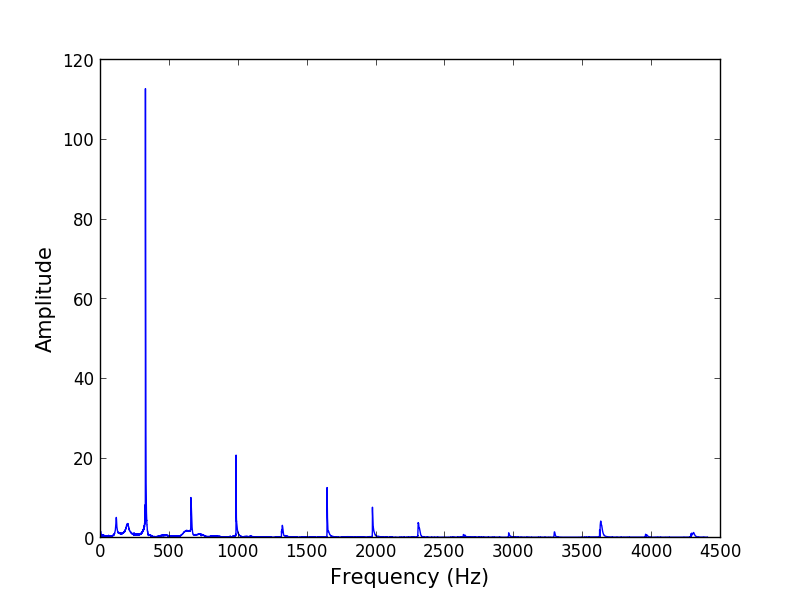
\includegraphics[width=\textwidth]{figures/freqanal/single_high.png}
\caption{$E_4$.}
\label{fig:single_high}
\end{subfigure}
\caption{Frequency spectra of $E_2$ and $E_4$ strings on a guitar. The harmonics are clearly visible.}
\label{fig:single}
\end{figure}
With a peak detection algorithm implemented in Python the most significant frequencies in the two recordings are registered to be 163.82 Hz and 329.83 Hz for $E_2$ and $E_4$, respectively. As $163.82$ Hz $\approx 2\cdot82.41$ Hz this is regarded as a harmonic of $E_2$. The harmonics are moreover observable in the figures as reduced peaks at integer multiples of the fundamental frequencies of the tones. It is furthermore seen from the figures, that the energy in the signals is mainly located at frequencies above 75 Hz and below 1000 Hz for $E_2$ and above 100 Hz and below 2000 Hz for $E_4$.\\ 

\subsection{Chord}
Figures \ref{fig:chord_low} and \ref{fig:chord_high} show the frequency spectra of the recordings of  $E_2$ and $E_4$ chords, respectively.
\begin{figure}[H]
\centering
\begin{subfigure}{0.49\textwidth}
\centering
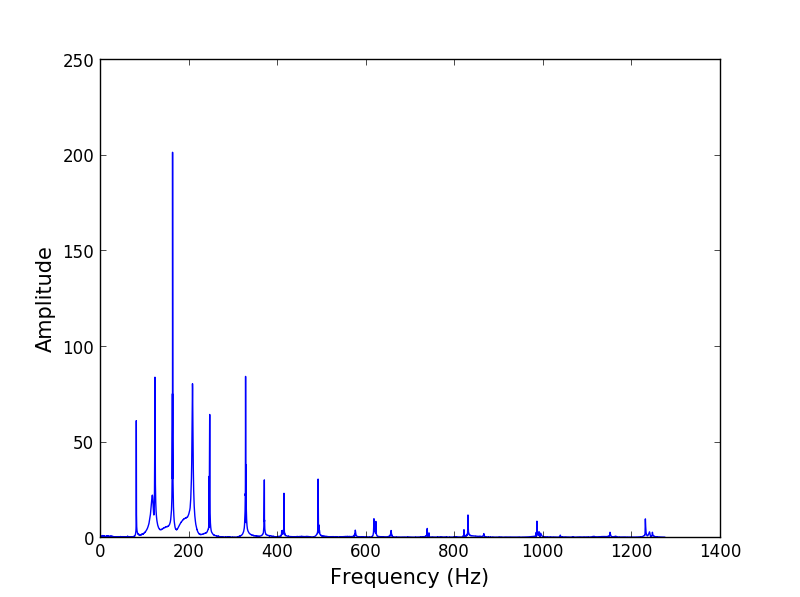
\includegraphics[width=0.9\textwidth]{figures/freqanal/chord_low.png}
\caption{$E_2$ chord.}
\label{fig:chord_low}
\end{subfigure}
\begin{subfigure}{0.49\textwidth}
\centering
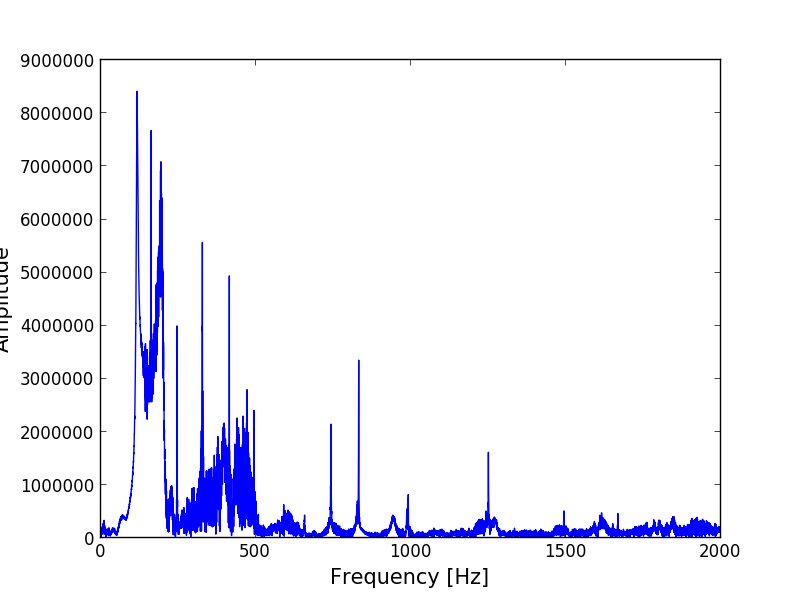
\includegraphics[width = 0.9\textwidth]{figures/freqanal/chord_high.png}
\caption{$E_4$ chord.}
\label{fig:chord_high}
\end{subfigure}
\caption{Frequency spectra of $E_2$ and $E_4$ chords played on a guitar.}
\label{fig:chord}
\end{figure}

The most significant frequencies in figure \ref{fig:chord_low} is 163.86 Hz and 119.27 Hz in figure \ref{fig:chord_high}. Once again it is assumed that the higher frequency of $E_2$ is due to harmonics. The second frequency does furthermore not correspond to a specific tone, and this is assumed to be because of the composition of chords being of multiple tones. The majority of the energy in the signals is located above 80 Hz and below 1000 Hz.
\subsection{Scale}
Figure \ref{fig:scale_fast} shows the frequency spectrum of a natural minor scale.
\begin{figure}[H]
\centering
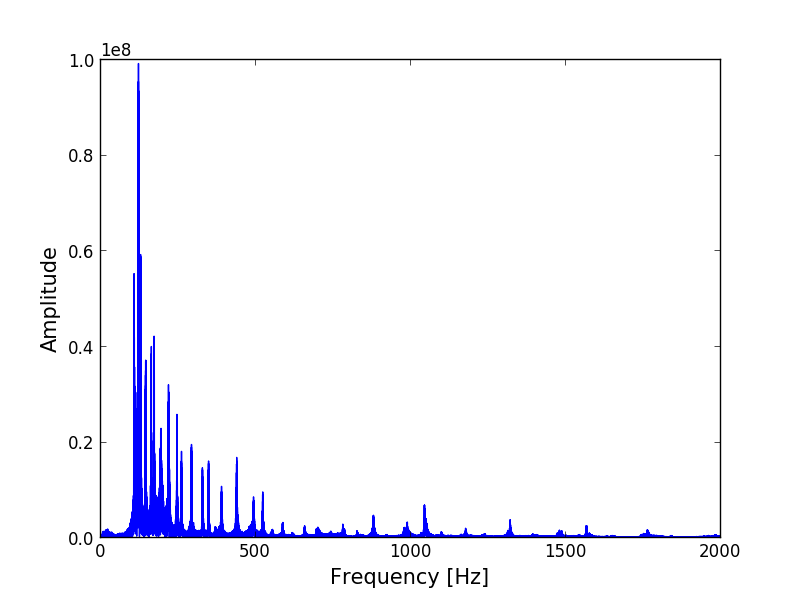
\includegraphics[width=0.7\textwidth]{figures/freqanal/scale_fast.png}
\caption{Frequency spectrum of the natural minor scale with root on 6th string played from the 6th fret.}
\label{fig:scale_fast}
\end{figure}
The scale includes tones of frequencies from 116.54 Hz to 554.36 Hz. As seen in the spectrum the majority of the energy in the signal is located above 100 Hz and below 600 Hz.

\subsection{Melody with single tones}
Figure \ref{fig:melody_single} shows the frequency spectrum for Itsy Bitsy Spider played slowly and only with single tones.
\begin{figure}[H]
\centering
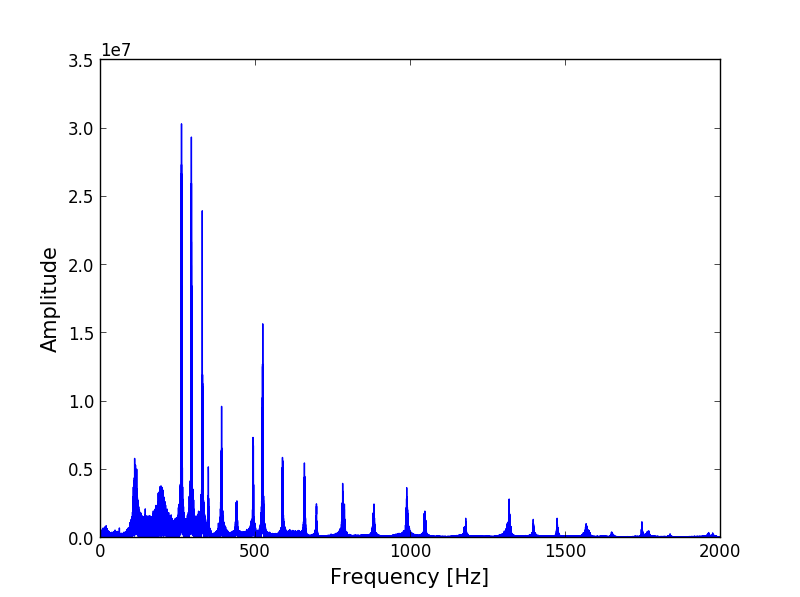
\includegraphics[width=0.7\textwidth]{figures/freqanal/melody_single.png}
\caption{Frequency spectrum of Itsy Bitsy Spider played on a guitar with only single strings plucked.}
\label{fig:melody_single}
\end{figure}
The majority of energy in the signal is located above 100 Hz and below 2000 Hz.

\section{Frequency analysis of noise}
In this section the recordings of noise will undergo frequency analyses, and the goal is to be able to express which frequencies the recorded noise are generally found at.
\subsection{Folding paper and clapping}
Figure \ref{fig:clapping} and \ref{fig:folding} show the frequency spectrum of clapping at equidistant intervals in time and folding a piece of paper, respectively.
\begin{figure}[H]
\centering
\begin{subfigure}{0.49\textwidth}
\centering
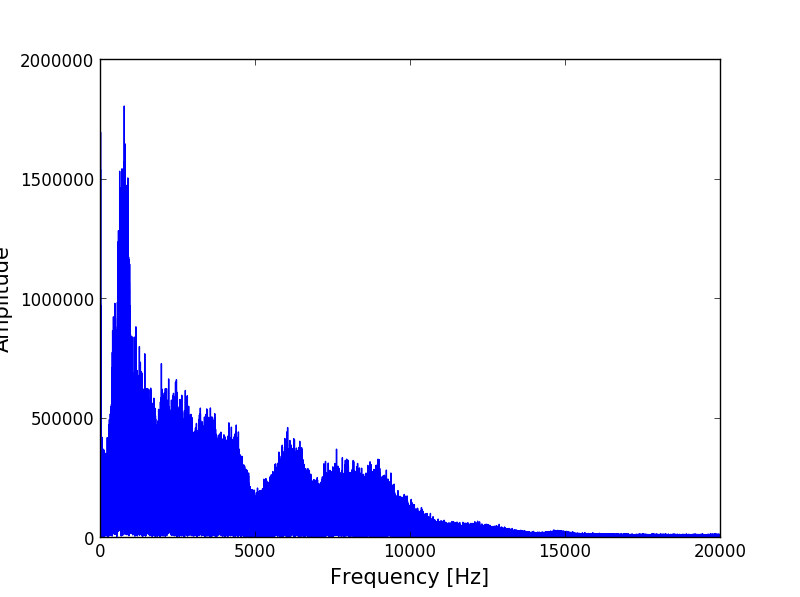
\includegraphics[width=\textwidth]{figures/freqanal/clapping.png}
\caption{}
\label{fig:clapping}
\end{subfigure}
\begin{subfigure}{0.49\textwidth}
\centering
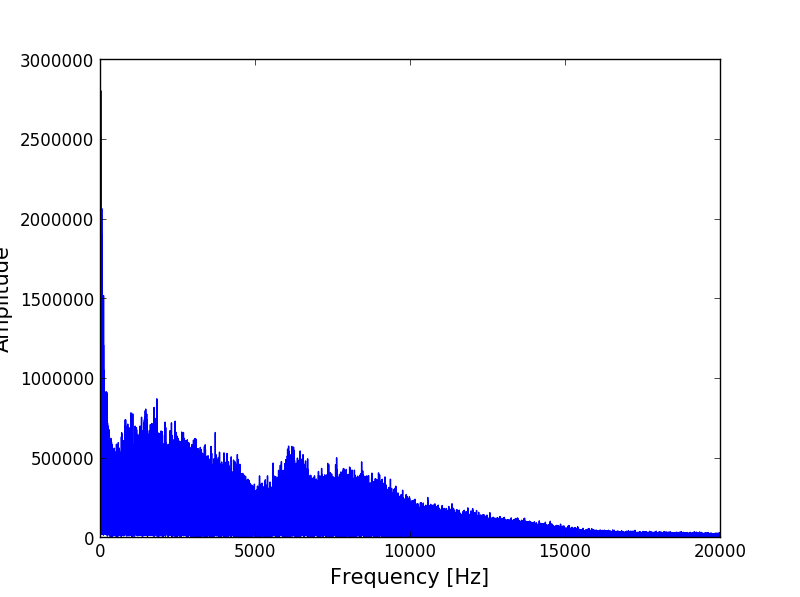
\includegraphics[width=\textwidth]{figures/freqanal/folding.png}
\caption{}
\label{fig:folding}
\end{subfigure}
\caption{Frequency spectra of \textbf{(a)} clapping at equidistant intervals and \textbf{(b)} folding a piece of paper.}
\end{figure}
The majority of the energy in both noises is located between 0 and 15000 Hz.
%\subsection{Singing and talking}
%Figures \ref{fig:talk} and \ref{fig:song} show the frequency spectrum of recorded talking and singing respectively.
%\begin{figure}[H]
%\centering
%\begin{subfigure}{0.49\textwidth}
%\centering
%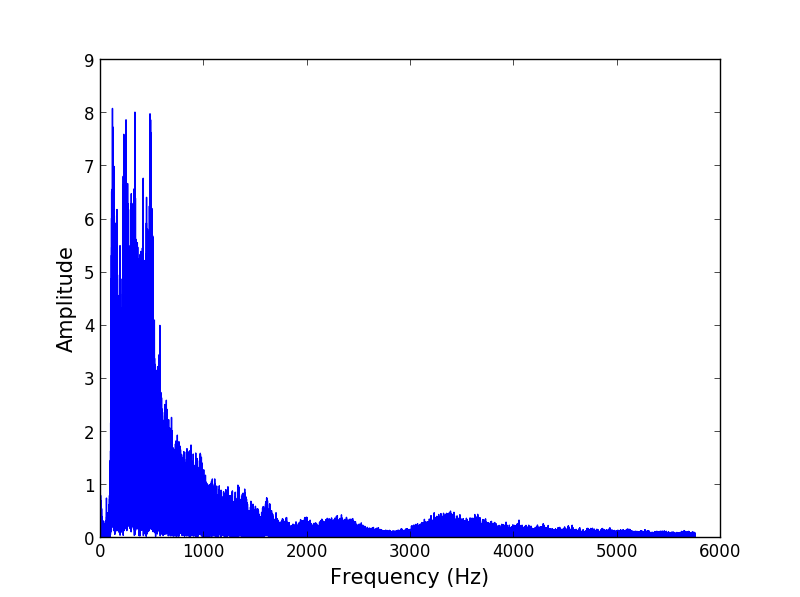
\includegraphics[width=\textwidth]{figures/freqanal/talk.png}
%\caption{Person talking}
%\label{fig:talk}
%\end{subfigure}
%\begin{subfigure}{0.49\textwidth}
%\centering
%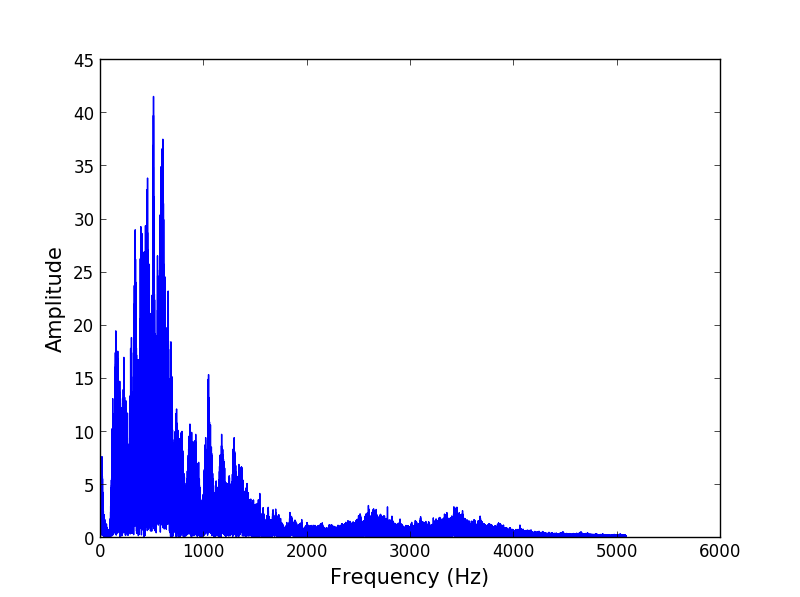
\includegraphics[width=\textwidth]{figures/freqanal/song.png}
%\caption{Person singing}
%\label{fig:song}
%\end{subfigure}
%\caption{Frequency spectra of a person talking and signing.}
%\end{figure}
%The majority of the energy is located between 100 and 5000 Hz for talking and 0 and 5000 Hz for singing.
\subsection{Ambient noise}
Figure \ref{fig:ambient} shows the frequency spectrum of the ambient noise recorded in a parking lot at the campus of AAU.
\begin{figure}[H]
\centering
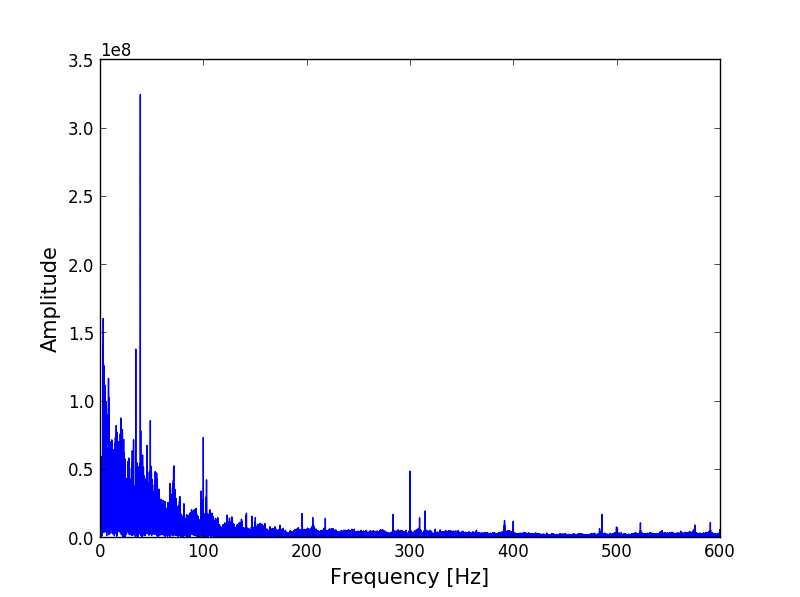
\includegraphics[width=0.7\textwidth]{figures/freqanal/ambient.png}
\caption{Frequency spectrum for ambient sound.}
\label{fig:ambient}
\end{figure}
The majority of the energy in the signal is located between 0 and 250 Hz.











